\documentclass[hidelinks]{ctexart}

\usepackage{van-de-la-illinoise}
\usepackage[paper=b5paper,top=.3in,left=.9in,right=.9in,bottom=.3in]{geometry}
\usepackage{calc}
\pagenumbering{gobble}
\setlength{\parindent}{0pt}
\sisetup{inter-unit-product=\ensuremath{{}\cdot{}}}
\usepackage{van-le-trompe-loeil}
\usetikzlibrary{quotes,angles}
\usepackage{makecell}

\usepackage{stackengine}
\stackMath
\usepackage{scalerel}
\usepackage[outline]{contour}

\newdimen\indexlen
\def\newprobheader#1{%
\def\probindex{#1}
\setlength\indexlen{\widthof{\textbf{\probindex}}}
\hskip\dimexpr-\indexlen-1em\relax
\textbf{\probindex}\hskip1em\relax
}
\def\newprob#1{%
\newprobheader{#1}%
\def\newprob##1{%
\probsep%
\newprobheader{##1}%
}%
}
\def\probsep{\vskip1em\relax{\color{gray}\dotfill}\vskip1em\relax}

\newlength\thisletterwidth
\newlength\gletterwidth
\newcommand{\leftrightharpoonup}[1]{%
{\ooalign{$\scriptstyle\leftharpoonup$\cr%\kern\dimexpr\thisletterwidth-\gletterwidth\relax
$\scriptstyle\rightharpoonup$\cr}}\relax%
}
\def\tensor#1{\settowidth\thisletterwidth{$\mathbf{#1}$}\settowidth\gletterwidth{$\mathbf{g}$}\stackon[-0.1ex]{\mathbf{#1}}{\boldsymbol{\leftrightharpoonup{#1}}}  }
\def\onedot{$\mathsurround0pt\ldotp$}
\def\cddot{% two dots stacked vertically
  \mathbin{\vcenter{\baselineskip.67ex
    \hbox{\onedot}\hbox{\onedot}}%
}}%

\begin{document}

\newprob{2.4}%
由对称性仅保留$\sin n\theta$项,
\[ \varphi\pare{r,\theta} = \begin{cases}
    \displaystyle \sum_{n=1}^\infty A_0 \frac{r^n}{a^n} \sin n\theta, & r<a, \\
    \displaystyle \sum_{n=1}^\infty B_0 \frac{a^n}{r^n} \sin n\theta, & r>a.
\end{cases} \]
由电势的连续性知$A_0 = B_0$, 边界条件要求
\[ \sum_{n=1}^\infty A_n \sin\theta = \varphi_{r=a} = \begin{cases}
    V, & 0 < \phi < \pi,\\
    -V, & -\pi < \phi < 0.
\end{cases} \]
从而
\[ A_n = \rec{\pi}\int_{-\pi}^{\pi} \varphi_{r=a}\cdot \sin n\theta\,\rd{\theta} = \begin{cases}
    \displaystyle \frac{4V_0}{n\pi}, & \text{\color{lightgray}\texttt{if (n \% 2)}}, \\
    \displaystyle 0, & \text{\color{lightgray}\texttt{if (!(n \% 2))}}.
\end{cases} \]
故
\[ \boxed{\varphi\pare{r,\theta} = \begin{cases}
    \displaystyle \frac{4V_0}{\pi}\sum_{n=1,3,5,\cdots} \rec{n}\frac{r^n}{a^n} \sin n\theta, & r<a, \\[.5em]
    \displaystyle \frac{4V_0}{\pi}\sum_{n=1,3,5,\cdots} \rec{n}\frac{a^n}{r^n} \sin n\theta, & r>a.
\end{cases}} \]
\par
\newprobheader{注}%
取保形变换$\displaystyle w = \frac{a-z}{z+a}$, 求解区域发生如下变化.\\
\centerline{%
    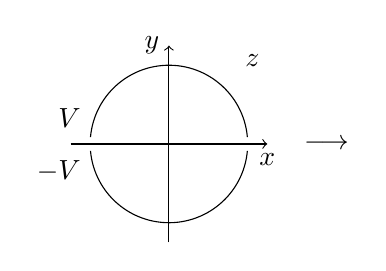
\begin{tikzpicture}[scale=0.5]
        \draw (5:2) arc (5:175:2) node[above left]{$V$};
        \draw (-5:2) arc (-5:-175:2) node[below left]{$-V$};
        \draw[->] (-2.5,0) -- (2.5,0) node[below]{$x$};
        \draw[->] (0,-2.5) -- (0,2.5) node[left]{$y$};
        \draw (45:3) node {$z$};
        \draw (4,0) node{$\longrightarrow$};
    \end{tikzpicture}
    \begin{tikzpicture}[scale=0.5]
        \draw[->] (0,0) -- (3.5,0) node[below]{$u$};
        \draw[->] (0,-2.5) -- (0,-1.25) node[left]{$V$} -- (0,-0.1) (0,0.1) -- (0,1.25) node[left]{$-V$} -- (0,2.5) node[left]{$v$};
        \draw (45:3) node {$w$};
    \end{tikzpicture}
}
注意到$\displaystyle f\pare{w} = -\frac{2 V}{\pi}\ln w$是解析函数, 故$\displaystyle \Im f\pare{w} = -\frac{2V}{\pi}\arg w$是调和函数且满足边界条件. 故$\displaystyle \varphi\pare{z} = -\frac{2V}{\pi}\arg \frac{a-z}{z+a} = \frac{2V}{\pi}\arctan\pare{\frac{2ay}{a^2-r^2}}$是原问题的解. 由反演变换保持调和性可得外部的解.
\[ \boxed{\varphi\pare{r,\theta} = \begin{cases}
    \displaystyle \frac{2V}{\pi}\arctan\pare{\frac{2\pare{r/a}\sin\phi}{1-\pare{r/a}^2}}, & r<a, \\
    \displaystyle \frac{2V}{\pi}\arctan\pare{\frac{2\pare{a/r}\sin\phi}{1-\pare{a/r}^2}}, & r>a.
\end{cases}} \]
\newprob{2.5}%
以$\+vE_0$方向为$z$轴, 可设外部
\[ \varphi = -E_0 r\cos\theta + \sum_{n=0}^\infty A_n \pare{\rec{r}}^{n+1}P_n\pare{\cos\theta}. \]
其中$\displaystyle A_0 = \frac{Q}{4\pi \epsilon_0}$, $A_1$须满足
\[ E_0 a \cos\theta = A_1 \rec{a^2} \cos\theta \Rightarrow A_1 = E_0 a^3. \]
其余$A_n = 0$. 故
\begin{align*}
    \varphi &= -E_0 r\cos\theta + \frac{Q}{4\pi\epsilon_0 r} + \frac{E_0a^3}{r^2} \cos\theta = -\+vE_0 \cdot \+vr + \frac{Q}{4\pi \epsilon_0 r} + \frac{\+vE_0 a^3 \cdot \+ur}{r^2}. \\
    \+vE &= \+vE_0 + \frac{Q\+ur}{4\pi\epsilon_0 r^2} - \frac{a^3}{r^3}\pare{\+vE_0 - 3\pare{\+vE_0\cdot \+ur}\+ur}. \\
    \left.\+vE\right\vert_{r=a} &= \pare{\frac{Q}{4\pi\epsilon_0 a^2} + 3E_0\cos\theta} \+vr.\\
    \+vF &= \frac{\+uz}{2} \iint \rd{\sigma} \, \epsilon_0 E^2\cos\theta = \+uz \pi \int_0^{\pi/2} \rd{\theta}\, a^2 \sin\theta\cdot \cos\theta \cdot \epsilon_0 \pare{\frac{Q}{4\pi\epsilon_0 a^2} + 3E_0\cos\theta}^2 \\
    &= \boxed{\pare{\frac{Q^2}{32\pi\epsilon_0 a^2} + \half QE_0 + \frac{9}{4}\pi a^2\epsilon_0 E_0^2}\+uz.}
\end{align*}
\newprob{2.6}%
取$\+vp_0$的方向为$\+uz$方向, 设球内电势为
\[ \varphi_1 = \frac{p_0\cos\theta}{4\pi\epsilon_1 r^2} + \sum_{n=0}^\infty A_n \pare{\frac{r}{a}}^n P_n\pare{\cos\theta}, \]
球外电势为
\[ \varphi_2 = \sum_{n=0}^\infty B_n \pare{\frac{a}{r}}^{n+1}P_n\pare{\cos\theta}. \]
$r=a$处有
\begin{align*}
    & \left.\varphi_1\right\vert_{r=a} = \left.\varphi_2\right\vert_{r=a} \Rightarrow \begin{cases}
        \displaystyle \frac{p_0}{4\pi\epsilon_1 a^2} + A_1 = B_1, \\
        A_n = B_n, & n\neq 1.
    \end{cases} \\
    & \left.\epsilon_1 \+drd{\varphi_1} \right\vert_{r=a} = \left.\epsilon_2 \+drd{\varphi_2} \right\vert_{r=a} \Rightarrow \begin{cases}
        \displaystyle \epsilon_1 \pare{-\frac{p_0}{2\pi\epsilon_1 a^2} + A_1} = -2\epsilon_2 B_1, \\
        \epsilon_1 A_n n = \epsilon_2 B_n \pare{n+1}, & n>1.
    \end{cases} \\
    & \Rightarrow \begin{cases}
        \displaystyle A_1 = \frac{\epsilon_1 - \epsilon_2}{2\epsilon_2 + \epsilon_1} \frac{p_0}{2\pi\epsilon_0 a^2}, \\[.5em]
        \displaystyle B_1 = \frac{3\epsilon_1}{4\epsilon_2 + 2\epsilon_1} \frac{p_0}{2\pi\epsilon_0 a^2}.
    \end{cases} \\
    & \Rightarrow \boxed{\varphi = \begin{cases}
        \displaystyle \frac{p_0\cos\theta}{4\pi\epsilon_1 r^2} + \frac{\epsilon_1 - \epsilon_2}{2\epsilon_2 + \epsilon_1} \frac{p_0r \cos\theta}{2\pi\epsilon_1 a^3}, & r<a, \\[.5em]
        \displaystyle \frac{3}{2\epsilon_2 + \epsilon_1} \frac{p_0 \cos\theta}{4\pi r^2}, &r>a.
    \end{cases}}
\end{align*}
\newprob{2.7}%
\\[-2\baselineskip]
\begin{flalign*}
    \+vF &= \+vp \+v\cdot \grad \+vE\+_\text{外}_ = p\+DsD{\+vE\+_\text{外}_} &\\
    &= \+us\brac{\frac{4\pi a^3}{3}\cdot \frac{3\epsilon_0 \pare{\epsilon - \epsilon_0}}{\epsilon + 2\epsilon_0}E\+_\text{外}_ \+DsD{E\+_\text{外}_}} &\\
    &= -\+us \frac{4\pi a^3}{3}\frac{3\epsilon_0\pare{\epsilon-\epsilon_0}}{\epsilon+2\epsilon_0}\pare{\frac{\lambda}{2\pi \epsilon_0}}^2 \rec{s^3}   & \\
    &= \boxed{-\frac{\epsilon - \epsilon_0}{\epsilon+2\epsilon_0} \frac{a^3}{\epsilon_0 \pi}\frac{\lambda^2}{R^3}\+us.}
\end{flalign*}
这是外电场作用在诱导出的电偶极子上的力.
\newprob{2.8}%
设$O$点为区域中心, 则
\[ \varphi\pare{O} = -\epsilon_0 \oiint_{\partial V}\rd{\sigma'}\,\varphi\pare{\+vr'} \+D{n'}D{G_D\pare{O;\+vr'}} = - \sum_{n=1}^N \varphi_n \epsilon_0 \iint_{\text{面}n}\rd{\sigma'}\, \+D{n'}D{G_D\pare{O;\+vr'}}. \]
由Green函数为对单位电荷的响应及正多面体的对称性知
\[ -\epsilon_0 \iint_{\text{单个面}}\rd{\sigma'}\, \+D{n'}D{G_D\pare{O;\+vr'}} = -\rec{N} \epsilon_0 \oiint_{\partial V}\rd{\sigma'}\, \+D{n'}D{G_D\pare{O;\+vr'}} = \rec{N}. \]
从而
\[ \varphi\pare{O} = \rec{N}\sum_{n=1}^N \varphi_n. \]
\newprob{2.9}%
上半空间的Green函数满足
\[ -\epsilon_0 \+D{n'}D{G_D} = \frac{z}{2\pi \+gr^3}, \]
故
\[ \varphi\pare{x,y,z} = -\epsilon_0 \iint_{-a<x<a} \rd{\sigma'}\, \varphi\pare{\+vr'} \+D{n'}D{G_D\pare{\+vr;\+vr'}} = \frac{V}{2\pi} \iint_{-a<x<a} \frac{z}{\+gr^3}\,\rd{x}\,\rd{y}. \]
注意到积分式的形式和$\pare{-a<x<a}$的带状均匀电荷在$\pare{x,y,z}$产生电场的$z$分量形式相同,\\
\centerline{\begin{tikzpicture}
    \draw[->] (-2,0) -- (2,0) node[below] {$x$};
    \draw[->] (0,-0.5) -- (0,2) node[left] {$y$};
    \draw[line width=0.1em] (-1,0) node[below] {$-a$} -- (1,0) node[below] {$a$};
    \draw (1.5,1.5) node[circ] {$\ \pare{x,y}$};
    \draw (-1,0) -- (1.5,1.5) -- (1,0);
    \node at ($(1.5,1.5)+(-135:7mm)$) {$\Delta\theta$};
    \draw[dashed] (1.5,1.5) -- (-0.5,0) node[midway,anchor=north] {$s$};
\begin{scope}
    \path[clip] (-1,0) -- (1.5,1.5) -- (1,0);
    \draw (1.5,1.5) circle (3mm);
\end{scope}
\end{tikzpicture}}
从而
\[ \varphi\pare{x,y,z} = \frac{V}{2\pi}\cdot 2 \int_{-a}^{a}\,\rd{x}\, \frac{\cos\theta}{s} = \frac{V}{\pi}\Delta\theta. \]
其中
\[ \Delta \theta = \frac{\pi}{2} + \arctan\pare{\frac{a^2-x^2-y^2}{2ay}}. \]
故
\[ \boxed{\varphi = \frac{V}{2} + \frac{V}{\pi}\arctan\pare{\frac{a^2-x^2-y^2}{2ay}}.} \]
电场
\[ \+vE = -\grad \varphi = \boxed{\frac{V}{\pi}\frac{4axy}{\pare{2ay}^2 + \pare{a^2-x^2-y^2}^2}\+ux + \frac{V}{\pi}\frac{2a\pare{-x^2+y^2+a^2}}{\pare{2ay}^2 + \pare{a^2-x^2-y^2}^2}\+uy.} \]
\par
\newprobheader{注}%
取保形变换$\displaystyle w = \frac{ia-z}{z+ia}$, 则变为求解如下问题.\\
\centerline{%
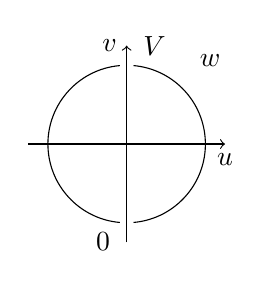
\begin{tikzpicture}[scale=0.5]
        \draw (-85:2) arc (-85:85:2) node[above right]{$V$};
        \draw (95:2) arc (95:265:2) node[below left]{$0$};
        \draw[->] (-2.5,0) -- (2.5,0) node[below]{$u$};
        \draw[->] (0,-2.5) -- (0,2.5) node[left]{$v$};
        \draw (45:3) node {$w$};
\end{tikzpicture}
}
由2.4的结果,
\[ \varphi = \frac{V}{2} + \frac{V}{\pi} \arg \frac{i\pare{a-z}}{a+z} = \frac{V}{2} + \frac{V}{\pi}\arctan\pare{\frac{a^2-x^2-y^2}{2ay}}. \]
\newprob{Pr 1 (a)}%
由系统的旋转对称性知$\varphi$与$\phi$无关. 球坐标系下电势有展开
\[ \varphi\pare{r} = \sum_{n=0}^\infty \pare{A_n r^n + \frac{B_n}{r^{n+1}}}\brac{C_n P_n\pare{\cos\theta} + D_n Q_n\pare{\cos\theta}}, \]
其中$P_n$和$Q_n$分别为第一类和第二类Legendre函数. 由$r=0$和$r\rightarrow \infty$时电势的非奇异知含有$r, r^2, \cdots$以及$\displaystyle \rec{r}, \rec{r^2}, \cdots$的项应排除, 故
\[ \varphi = \varphi\pare{\theta} = C_0 P_0\pare{\cos\theta} + D_0 Q_0\pare{\cos\theta}. \]
与$r$亦无关.
\par
\newprobheader{(b)}%
$\displaystyle \laplacian \varphi = 0 \Rightarrow \rec{r^2\sin\theta}\+D\theta D{}\pare{\sin\theta \+D{\theta}D{\varphi}} = 0$. 从而
\[ \sin \theta \+D{\theta}D\varphi = c_1 \Rightarrow \varphi = c_0 + c_1 \log \tan \frac{\theta}{2}. \]
由边界条件知
\[ \varphi\vert_{\theta = \pi/2} = 0 \Rightarrow c_0 = 0,\quad \varphi\vert_{\theta = \pi/4} = V \Rightarrow c_1 = \frac{V}{\ln \tan \pi/8}. \]
故
\[ \varphi = \boxed{\frac{\displaystyle V \ln \tan \frac{\theta}{2}}{\displaystyle \ln \tan \frac{\pi}{8}}.} \]
\newprob{Pr 2 (a)}%
观察得
\[ \+vE = -\frac{V_0}{R^3}\grad \pare{x^2y - \frac{y^3}{3} + V_0 zR^2} \Rightarrow \boxed{\varphi = \frac{V_0}{R^3} \pare{x^2y - \frac{y^3}{3} + zR^2}.} \]
\par
\newprobheader{(b)}%
转化为球坐标系, 有
\begin{align*}
    \varphi_1 &= V_0 \brac{\rec{3}\pare{\frac{r}{R}}^3 \sin^3\theta \sin 3\phi + \frac{r}{R}\cos\theta},\quad r<R.
\end{align*}
注意到$\displaystyle P_3^3\pare{\cos\theta} = -15\sin^3\theta$, $P_1^0\pare{\cos\theta} = \cos\theta$, $\varphi$已经是球坐标系下的调和函数展开的形式, 故$\pare{r/R}^n\mapsto \pare{R/r}^{n+1}$可以得到球外的解,
\begin{align*}
    \varphi_2 &= V_0 \brac{\rec{3}\pare{\frac{R}{r}}^4 \sin^3\theta \sin 3\phi + \pare{\frac{R}{r}}^2\cos\theta},\quad R>r.\\
    \sigma &= \epsilon_0 \pare{\+DrD{\varphi_1} - \+DrD{\varphi_2}}_{r=a} = \boxed{\frac{\epsilon_0 V_0}{R} \brac{\frac{7}{3} \sin^3\theta \sin 3\phi + 3 \cos\theta}.} \\
    \rho &= \boxed{0.}
\end{align*}
\newprob{Pr 3}%
设$\varphi$有展开
\[ \varphi = \begin{cases}
    \displaystyle \varphi_1 = \sum_{n=0}^\infty a_n \pare{\frac{r}{R}}^{n} \cos n\phi, & r<a,\\
    \displaystyle \varphi_2 = \sum_{n=0}^\infty b_n \pare{\frac{R}{r}}^n \cos n\phi + b_0 \ln \frac{r}{R}, & r>a.
\end{cases} \]
其中$\displaystyle b_0 = -\frac{\lambda}{2\pi\epsilon_0}$. 而$\varphi_1\vert_{r=R} = \varphi_2\vert_{r=R}$要求$a_n = b_n$. 故在存在导体的区域内
\[ \pare{-\+DrD{}\varphi_1\ - \+DrD{}\varphi_2}_{r=R} = -\frac{b_0}{R} = \frac{\Delta \sigma}{\epsilon_0} \Rightarrow -\frac{b_0}{R}\cdot 2\pi \pare{1-\rec{p}} = \frac{\Delta\lambda}{\epsilon_0}. \]
从而
\[ \lambda_{\text{内}} = \frac{\lambda}{2} - \frac{\Delta \lambda}{2} = \frac{\lambda}{2p} \Rightarrow \boxed{\frac{\lambda_{\text{内}}}{\lambda} = \rec{2p}.} \]
\par
\newprobheader{注}%
通过保形映射$\displaystyle w = \frac{z-R}{z+R}$, 区域发生如下变化.\\
\centerline{%
    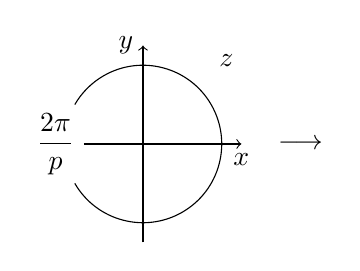
\begin{tikzpicture}[scale=0.5]
        \draw (-150:2) arc (-150:150:2) node[above left]{};
        \draw[->] (-1.5,0) -- (2.5,0) node[below]{$x$};
        \draw[->] (0,-2.5) -- (0,2.5) node[left]{$y$};
        \draw (-1.5,0) node[left] {$\displaystyle \frac{2\pi}{p}$};
        \draw (45:3) node {$z$};
        \draw (4,0) node{$\longrightarrow$};
    \end{tikzpicture}
    \begin{tikzpicture}[scale=0.5]
        \draw[->] (0,0) -- (3.5,0) node[below]{$u$};
        \draw[->] (0,-2.5) -- (0,-2) node[left]{$-a$} -- (0,2) node[left]{$a$} -- (0,2.5) node[left]{$v$};
        \draw[line width = 0.1em] (0,-2) -- (0,2);
        \draw (1,0) node[circ] {};
        \draw (1,0) node[below] {$1$};
        \draw (1,0) node[above] {$\ z=\infty$};
        \draw (45:3) node {$w$};
    \end{tikzpicture}
}
其中$\displaystyle a = \tan \frac{\pi\pare{p-1}}{2p}$. 为了求出$z$平面内的导体电势, 注意到$z=-R$被映射到$w=\infty$, 而$z=\infty$被映射到$w=1$. 为了得到在$z=-R$处非奇异且在$z=\infty$处渐进行为为$\ln \abs{z}$的解, 需要知道$w$平面内导体对$w=1$处电荷的响应. 这需要在$w$平面上求解
\[ \begin{cases}
    \laplacian \psi = 0,\\
    \displaystyle \psi\vert_{z\in \brac{-ia,ia}} = \half \ln \sqrt{1 + v^2}.
\end{cases} \]
若引入椭圆坐标$\pare{\mu,\nu}$满足
\[ \frac{a}{i}\cosh\pare{\mu + i\nu} = w, \]
则$\mu = 0$的坐标曲线恰好环绕导体表面. 椭圆坐标下在$\infty$处非奇异的的调和函数有展开
\[ \psi = \sum_{n=0}^\infty A_n \cos n\nu e^{-n\mu}. \]
若$e^{-\mu} \mapsto r$, $\nu \mapsto \theta$, 则该展开与极坐标系下的展开形式一致, $\mu = 0$对应$r=1$而$\mu = \infty$对应$r = 0$. 故有Poisson解
\[ \psi\pare{e^{-\mu - i\nu}} = \rec{2\pi} \int_{-\pi}^{\pi} \Re\pare{\frac{1+e^{-\mu - i\nu}e^{-it}}{1-e^{-\mu - i\nu}e^{-it}}}\cdot \half \ln \pare{1+a^2\cos^2 t}\,\rd{t}. \]
可得$z$平面上的解正比于
\[ \varphi = \mu + \psi - \log \abs{w - 1}. \]
若引入$\zeta = e^{-\mu - i\nu}$, 则
\[ \zeta = \frac{iw + \sqrt{-a^2 - w^2}}{a}. \]
其中$\sqrt{-a^2 - w^2}$以$\brac{-ia,ia}$为支割线, 并取$w\rightarrow\infty$时$\sqrt{-a^2 - w^2} \rightarrow -iw$的解析分支. 则
\[ \varphi = \begin{cases}
    -\Re \log \zeta\pare{z}\\ \displaystyle + \rec{2\pi} \int_{-\pi}^{\pi} \Re\pare{\frac{1+\zeta\pare{z}e^{-it}}{1-\zeta\pare{z}e^{-it}}}\cdot \half \ln \pare{1+a^2\cos^2 t}\,\rd{t}\\ - \log\abs{w\pare{z} - 1}.
\end{cases}  \]
\begin{figure}
    \centering
    \begin{subfigure}{.3\linewidth}
        \centering
        \includegraphics[width=\linewidth]{src/TrisectCylinder.pdf}
        \caption{$\pi/3$}
    \end{subfigure}
    \begin{subfigure}{.3\linewidth}
        \centering
        \includegraphics[width=\linewidth]{src/BisectCylinderConductor.pdf}
        \caption{$\pi/2$}
    \end{subfigure}
    \begin{subfigure}{.3\linewidth}
        \centering
        \includegraphics[width=\linewidth]{src/TwoThirdsCylinder.pdf}
        \caption{$2\pi/3$}
    \end{subfigure}
    \caption*{不同张角的等势面}
\end{figure}
可以发现导体边缘处等势线密度极大. 计算表明该处电场发散.

\end{document}
